% Séquence 1 : Les nombres relatifs
\setseqtitle{Les nombres relatifs}
\chapter{Les nombres relatifs}

\begin{objectifsbox}
À l'issue de la séquence, l'élève sera capable de :
\begin{itemize}
\item Multiplier et diviser des nombres relatifs en appliquant la règle des signes
\item Généraliser la règle des signes pour plusieurs facteurs
\item Identifier et utiliser les nombres inverses
\item Calculer des expressions numériques avec enchaînements d'opérations
\item Résoudre des problèmes utilisant les nombres relatifs
\end{itemize}
\end{objectifsbox}

\section{Rappel : Les nombres relatifs}

\begin{remarkbox}[Rappel de 5e]
Les nombres relatifs sont des nombres qui peuvent être positifs, négatifs ou nuls. Ils permettent de décrire des quantités au-dessus ou en dessous de zéro.
\end{remarkbox}

\subsection{Représentation et comparaison}

\begin{proprietebox}
Sur une droite graduée :
\begin{itemize}[label = \textbullet]
\item Les nombres positifs sont à droite de 0
\item Les nombres négatifs sont à gauche de 0
\item Plus un nombre est à droite, plus il est grand
\end{itemize}
\end{proprietebox}

\begin{examplebox}
\textbf{Comparer les nombres :} $-4 < -1 < 0 < 2 < 5$

\begin{center}
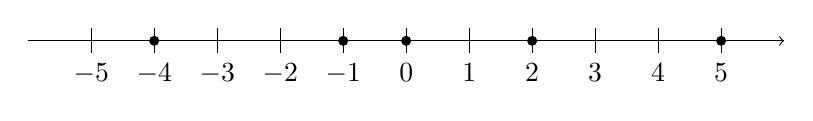
\begin{tikzpicture}[scale=0.8]
\draw[->] (-6,0) -- (6,0);
\foreach \x in {-5,-4,-3,-2,-1,0,1,2,3,4,5}
    \draw (\x,0.2) -- (\x,-0.2) node[below] {$\x$};
\draw[fill=black] (-4,0) circle (2pt);
\draw[fill=black] (-1,0) circle (2pt);
\draw[fill=black] (0,0) circle (2pt);
\draw[fill=black] (2,0) circle (2pt);
\draw[fill=black] (5,0) circle (2pt);
\end{tikzpicture}
\end{center}
\end{examplebox}

\subsection{Rappel : Addition et soustraction}

\begin{proprietebox}[Addition et soustraction]
\begin{itemize}[label = \textbullet]
\item \textbf{Même signe :} On additionne les distances à zéro et on garde le signe commun
\item \textbf{Signes différents :} On soustrait les distances à zéro et on garde le signe du nombre qui a la plus grande distance à zéro
\item \textbf{Soustraction :} Soustraire un nombre, c'est ajouter son opposé
\end{itemize}
\end{proprietebox}

\begin{examplebox}
\textbf{Exemples de calculs :}
\begin{align*}
(+5) + (+3) &= \trous{2.5cm} \\
(-4) + (-2) &= \trous{2.5cm} \\
(+7) + (-3) &= \trous{2.5cm} \\
(-5) + (+8) &= \trous{2.5cm} \\
(+6) - (+2) &= \trous{2.5cm} = \trous{2.5cm} \\
(-3) - (-5) &= \trous{2.5cm} = \trous{2.5cm}
\end{align*}
\end{examplebox}

\section{Multiplication et division de nombres relatifs}

\subsection{La règle des signes}

\begin{proprietebox}{Règle des signes}
\textbf{Règle des signes pour la multiplication et la division :}
\begin{itemize}[label = \textbullet]
\item $(+) \times (+) = (+)$ \quad et \quad $(+) \div (+) = (+)$
\item $(-) \times (-) = (+)$ \quad et \quad $(-) \div (-) = (+)$
\item $(+) \times (-) = (-)$ \quad et \quad $(+) \div (-) = (-)$
\item $(-) \times (+) = (-)$ \quad et \quad $(-) \div (+) = (-)$
\end{itemize}

\textbf{Méthode :} On détermine d'abord le signe du résultat, puis on calcule avec les distances à zéro.
\end{proprietebox}

\begin{examplebox}
\textbf{Calculer les produits et quotients suivants :}

\begin{minipage}[t]{0.48\textwidth}
\textbf{Multiplication :}
\begin{align*}
(+4) \times (+3) &= \trous{2cm} \\
(-5) \times (-2) &= \trous{2cm} \\
(+6) \times (-3) &= \trous{2cm} \\
(-7) \times (+4) &= \trous{2cm}
\end{align*}
\end{minipage}
\hfill
\begin{minipage}[t]{0.48\textwidth}
\textbf{Division :}
\begin{align*}
(+15) \div (+3) &= \trous{2cm} \\
(-20) \div (-4) &= \trous{2cm} \\
(+24) \div (-6) &= \trous{2cm} \\
(-35) \div (+7) &= \trous{2cm}
\end{align*}
\end{minipage}
\end{examplebox}

\section{Généralisation de la règle des signes}

\subsection{Produit de plusieurs facteurs}

\begin{proprietebox}{Produit de plusieurs facteurs}
\textbf{Pour un produit de plusieurs facteurs :}
\begin{itemize}[label = \textbullet]
\item Si le nombre de facteurs négatifs est \textbf{pair}, le résultat est \textbf{positif}
\item Si le nombre de facteurs négatifs est \textbf{impair}, le résultat est \textbf{négatif}
\end{itemize}
\end{proprietebox}

\begin{examplebox}
\textbf{Déterminer le signe des produits suivants :}
\begin{itemize}[label = \textbullet]
\item $A = (-2) \times (+3) \times (-4) \times (-1)$ : \trous{2.5cm} facteurs négatifs, donc $A$ est \trous{2cm}
\item $B = (+5) \times (-2) \times (-3) \times (+1) \times (-4)$ : \trous{2.5cm} facteurs négatifs, donc $B$ est \trous{2cm}
\item $C = (-1) \times (-2) \times (-3) \times (-4)$ : \trous{2.5cm} facteurs négatifs, donc $C$ est \trous{2cm}
\end{itemize}
\end{examplebox}

\subsection{Nombres inverses}

\begin{definitionbox}{Nombres inverses}
Deux nombres relatifs sont des \textbf{nombres inverses} si leur produit est égal à 1. Soit $a$ et $b$ deux nombres relatifs. $a$ et $b$ sont dits « inverses » si et seulement si $a \times b = 1$.
\end{definitionbox}

\begin{examplebox}
\begin{itemize}[label = \textbullet]
\item L'inverse de 5 est \trous{1cm} car $5 \times \trous{1cm} = 1$
\item L'inverse de $-\frac{2}{3}$ est \trous{1cm} car $-\frac{2}{3} \times$ \trous{1cm} = 1
\item L'inverse de -4 est \trous{1cm} car $-4 \times$ \trous{1cm} = 1
\end{itemize}
\end{examplebox}

\section{Expressions numériques et enchaînements d'opérations}
\begin{methodebox}{Calcul d'expression numérique}
\textbf{Pour calculer une expression numérique :}
\begin{enumerate}[label = \arabic*)]
\item On effectue en premier les calculs dans les \textbf{parenthèses les plus intérieures}
\item On calcule les \textbf{puissances} éventuelles
\item On effectue ensuite les \textbf{multiplications et divisions} avant les additions et soustractions
\item Si plusieurs multiplications/divisions se suivent, on calcule dans le \textbf{sens de la lecture}
\item Si plusieurs additions/soustractions se suivent, on calcule dans le \textbf{sens de la lecture}
\end{enumerate}
\end{methodebox}

\begin{examplebox}
\textbf{Calculer les expressions suivantes :}

\noindent
\begin{minipage}[t]{0.48\textwidth}
\begin{align*}
A &= 5 + 3 \times (-2) \\
  &= \trous{2.5cm} \\
  &= \trous{2.5cm}
\end{align*}
\end{minipage}
\hfill
\begin{minipage}[t]{0.48\textwidth}
\begin{align*}
B &= (-8) \div 2 + 3 \times (-1) \\
  &= \trous{2.5cm} \\
  &= \trous{2.5cm}
\end{align*}
\end{minipage}

\vspace{1em}

\noindent
\begin{minipage}[t]{0.48\textwidth}
\begin{align*}
C &= [(-6) + 4] \times (-2) \\
  &= \trous{2.5cm} \\
  &= \trous{2.5cm}
\end{align*}
\end{minipage}
\hfill
\begin{minipage}[t]{0.48\textwidth}
\begin{align*}
D &= 12 \div (-3) \times 2 \\
  &= \trous{2.5cm} \\
  &= \trous{2.5cm}
\end{align*}
\end{minipage}
\end{examplebox}

\section{Exercices d'application}

\begin{exercisebox}
\textbf{Exercice 1 :} Calculs avec les nombres relatifs

Calculer les expressions suivantes :
\begin{enumerate}[label=\alph*)]
\item $(-3) \times (+4) \times (-2)$
\item $(+15) \div (-3) \times (-2)$
\item $[(-5) + (+3)] \times (-4)$
\item $(+8) \div (-2) + (-3) \times (+2)$
\end{enumerate}

\textbf{Exercice 2 :} Déterminer le signe

Sans faire le calcul, déterminer le signe des produits suivants :
\begin{enumerate}[label=\alph*)]
\item $(-2) \times (+3) \times (-4) \times (-1) \times (+5)$
\item $(+1) \times (-2) \times (-3) \times (+4) \times (-5)$
\item $(-1) \times (-2) \times (-3) \times (-4) \times (-5)$
\end{enumerate}

\textbf{Exercice 3 :} Nombres inverses

Trouver l'inverse de chacun des nombres suivants :
\begin{enumerate}[label=\alph*)]
\item 7
\item -3
\item $\frac{1}{4}$
\item $-\frac{2}{5}$
\end{enumerate}

\textbf{Exercice 4 :} Expressions complexes

Calculer les expressions suivantes en respectant les priorités :
\begin{enumerate}[label=\alph*)]
\item $(-6) \times (+2) + (-8) \div (-4)$
\item $[(-3) + (+5)] \times (-2) - (+4)$
\item $(+12) \div (-3) \times (+2) + (-5)$
\item $(-10) \div (+2) - (-3) \times (-4)$
\end{enumerate}
\end{exercisebox}

